\documentclass[journal,11pt]{IEEEtran}
%
\makeatletter
\makeatother
\usepackage{setspace}
\usepackage{gensymb}
\usepackage{xcolor}
\usepackage{caption}
%\usepackage{stackengine}
%\usepackage{subcaption}
%\doublespacing
\singlespacing



\usepackage{graphicx}
\graphicspath{ {./images}  }
%\usepackage{amssymb}
%\usepackage{relsize}
\usepackage[cmex10]{amsmath}
\usepackage{mathtools}
%\usepackage{amsthm}
\interdisplaylinepenalty=2500
%\savesymbol{iint}
%\usepackage{txfonts}
%\restoresymbol{TXF}{iint}
\usepackage{wasysym}
\usepackage{amsthm}
\usepackage{mathrsfs}
\usepackage{txfonts}
\usepackage{stfloats}
\usepackage{cite}
\usepackage{cases}
\usepackage{mathtools}
\usepackage{subfig}
\usepackage{enumerate}	
\usepackage{enumitem}
\usepackage{amsmath}
%\usepackage{xtab}
\usepackage{longtable}
\usepackage{multirow}
%\usepackage{algorithm}
%\usepackage{algpseudocode}
\usepackage{enumitem}
\usepackage{mathtools}
\usepackage[colorlinks=true, allcolors=blue]{hyperref}
%\usepackage{iithtlc}
\usepackage{tikz}
\usetikzlibrary{shapes,arrows}

%\usetikzlibrary{arrows.meta,calc,positioning}
%\usepackage[framemethod=tikz]{mdframed}
\usepackage{listings}
    \usepackage[latin1]{inputenc}                                 %%
    \usepackage{color}                                            %%
    \usepackage{array}                                            %%
    \usepackage{longtable}                                        %%
    \usepackage{calc}                                             %%
    \usepackage{multirow}                                         %%
    \usepackage{hhline}                                           %%
    \usepackage{ifthen}                                           %%
  %optionally (for landscape tables embedded in another document): %%
    \usepackage{lscape}     


%\usepackage{stmaryrd}


%\usepackage{wasysym}
%\newcounter{MYtempeqncnt}
\DeclareMathOperator*{\Res}{Res}
%\renewcommand{\baselinestretch}{4}
%\setcounter{secnumdepth}{4}
\renewcommand\thesection{\arabic{section}}
\renewcommand\thesubsection{\thesection.\arabic{subsection}}
\renewcommand\thesubsubsection{\thesubsection.\arabic{subsubsection}}
%\renewcommand\thesubsubsubsection{\thesubsubsection.\arabic{subsubsubsection}}

%\renewcommand\thesectiondis{\arabic{section}}
%\renewcommand\thesubsectiondis{\thesectiondis.\arabic{subsection}}
%\renewcommand\thesubsubsectiondis{\thesubsectiondis.\arabic{subsubsection}}
%\renewcommand\thesubsubsubsectiondis{\thesubsubsectiondis.\arabic{subsubsubsection}}
% correct bad hyphenation here
\hyphenation{Future Wireless communications}

%\lstset{
%language=C,
%frame=single, 
%breaklines=true
%}

%\lstset{
	%%basicstyle=\small\ttfamily\bfseries,
	%%numberstyle=\small\ttfamily,
	%language=Octave,
	%backgroundcolor=\color{white},
	%%frame=single,
	%%keywordstyle=\bfseries,
	%%breaklines=true,
	%%showstringspaces=false,
	%%xleftmargin=-10mm,
	%%aboveskip=-1mm,
	%%belowskip=0mm
%}

%\surroundwithmdframed[width=\columnwidth]{lstlisting}
\def\inputGnumericTable{}                                 %%

\lstset{
%language=python,
frame=single, 
breaklines=true,
columns=fullflexible
}

 

\begin{document}
%
\tikzstyle{block} = [rectangle, draw,
text width=7em, text centered, minimum height=4em]
\tikzstyle{sum} = [draw, circle, node distance=3cm]
\tikzstyle{input} = [coordinate]
\tikzstyle{output} = [coordinate]
\tikzstyle{pinstyle} = [pin edge={to-,thin,black}]
\tikzstyle{line} = [draw, -latex']
\theoremstyle{definition}
\newtheorem{theorem}{Theorem}[section]
\newtheorem{problem}{Problem}
\newtheorem{proposition}{Proposition}[section]
\newtheorem{lemma}{Lemma}[section]
\newtheorem{corollary}[theorem]{Corollary}
\newtheorem{example}{Example}[section]
\newtheorem{definition}{Definition}[section]
%\newtheorem{algorithm}{Algorithm}[section]
%\newtheorem{cor}{Corollary}
\newcommand{\BEQA}{\begin{eqnarray}}
\newcommand{\EEQA}{\end{eqnarray}}
\newcommand{\define}{\stackrel{\triangle}{=}}
\bibliographystyle{IEEEtran}
%\bibliographystyle{ieeetr}
\providecommand{\nCr}[2]{\,^{#1}C_{#2}} % nCr
\providecommand{\nPr}[2]{\,^{#1}P_{#2}} % nPr
\providecommand{\mbf}{\mathbf}
\providecommand{\pr}[1]{\ensuremath{\Pr\left(#1\right)}}
\providecommand{\qfunc}[1]{\ensuremath{Q\left(#1\right)}}
\providecommand{\sbrak}[1]{\ensuremath{{}\left[#1\right]}}
\providecommand{\lsbrak}[1]{\ensuremath{{}\left[#1\right.}}
\providecommand{\rsbrak}[1]{\ensuremath{{}\left.#1\right]}}
\providecommand{\brak}[1]{\ensuremath{\left(#1\right)}}
\providecommand{\lbrak}[1]{\ensuremath{\left(#1\right.}}
\providecommand{\rbrak}[1]{\ensuremath{\left.#1\right)}}
\providecommand{\cbrak}[1]{\ensuremath{\left\{#1\right\}}}
\providecommand{\lcbrak}[1]{\ensuremath{\left\{#1\right.}}
\providecommand{\rcbrak}[1]{\ensuremath{\left.#1\right\}}}
\theoremstyle{remark}
\newtheorem{rem}{Remark}
\newcommand{\sgn}{\mathop{\mathrm{sgn}}}
\providecommand{\abs}[1]{\left\vert#1\right\vert}
\providecommand{\res}[1]{\Res\displaylimits_{#1}} 
\providecommand{\norm}[1]{\lVert#1\rVert}
\providecommand{\mtx}[1]{\mathbf{#1}}
\providecommand{\mean}[1]{E\left[ #1 \right]}
\providecommand{\fourier}{\overset{\mathcal{F}}{ \rightleftharpoons}}
%\providecommand{\hilbert}{\overset{\mathcal{H}}{ \rightleftharpoons}}
\providecommand{\system}{\overset{\mathcal{H}}{ \longleftrightarrow}}
	%\newcommand{\solution}[2]{\textbf{Solution:}{#1}}
\newcommand{\solution}{\noindent \textbf{Solution: }}
\newcommand{\myvec}[1]{\ensuremath{\begin{pmatrix}#1\end{pmatrix}}}
\providecommand{\dec}[2]{\ensuremath{\overset{#1}{\underset{#2}{\gtrless}}}}
\DeclarePairedDelimiter{\ceil}{\lceil}{\rceil}
%\numberwithin{equation}{subsection}
\numberwithin{equation}{section}
%\numberwithin{problem}{subsection}
%\numberwithin{definition}{subsection}
%\makeatletter
%\@addtoreset{figure}{section}
%\makeatother
\let\StandardTheFigure\thefigure
%\renewcommand{\thefigure}{\theproblem.\arabic{figure}}
%\renewcommand{\thefigure}{\thesection}
%\numberwithin{figure}{subsection}
%\numberwithin{equation}{subsection}
%\numberwithin{equation}{section}
%\numberwithin{equation}{problem}
%\numberwithin{problem}{subsection}
%\numberwithin{problem}{section}
%%\numberwithin{definition}{subsection}
%\makeatletter
%\@addtoreset{figure}{problem}
%\makeatother
%\makeatletter
%\@addtoreset{table}{problem}
%\makeatother
\let\StandardTheFigure\thefigure
\let\StandardTheTable\thetable
\let\vec\mathbf
%%\renewcommand{\thefigure}{\theproblem.\arabic{figure}}
%\renewcommand{\thefigure}{\theproblem}
%%\numberwithin{figure}{section}
%%\numberwithin{figure}{subsection}
\def\putbox#1#2#3{\makebox[0in][l]{\makebox[#1][l]{}\raisebox{\baselineskip}[0in][0in]{\raisebox{#2}[0in][0in]{#3}}}}
     \def\rightbox#1{\makebox[0in][r]{#1}}
     \def\centbox#1{\makebox[0in]{#1}}
     \def\topbox#1{\raisebox{-\baselineskip}[0in][0in]{#1}}
     \def\midbox#1{\raisebox{-0.5\baselineskip}[0in][0in]{#1}}
\title{ 
%	\logo{
8085 Micro-Processor with ESP32  
%	}
}
\author{YADATI KRISHNA }% <-this % stops a space
% make the title area
\maketitle
%\tableofcontents

\section{\textbf{Intoduction}}
The 8085 microprocessor is an 8-bit microprocessor that was developed by Intel in the mid-1970s. It was widely used in the early days of personal computing and was a popular choice for hobbyists and enthusiasts due to its simplicity and ease of use. The architecture of the 8085 microprocessor consists of several key components, including the accumulator, registers, program counter, stack pointer, instruction register, flags register, data bus, address bus, and control bus.
The accumulator is an 8-bit register that is used to store arithmetic and logical results. It is the most commonly used register in the 8085 microprocessor and is used to perform arithmetic and logical operations such as addition, subtraction, and bitwise operations.\\

\begin{figure}[htb]
\centering
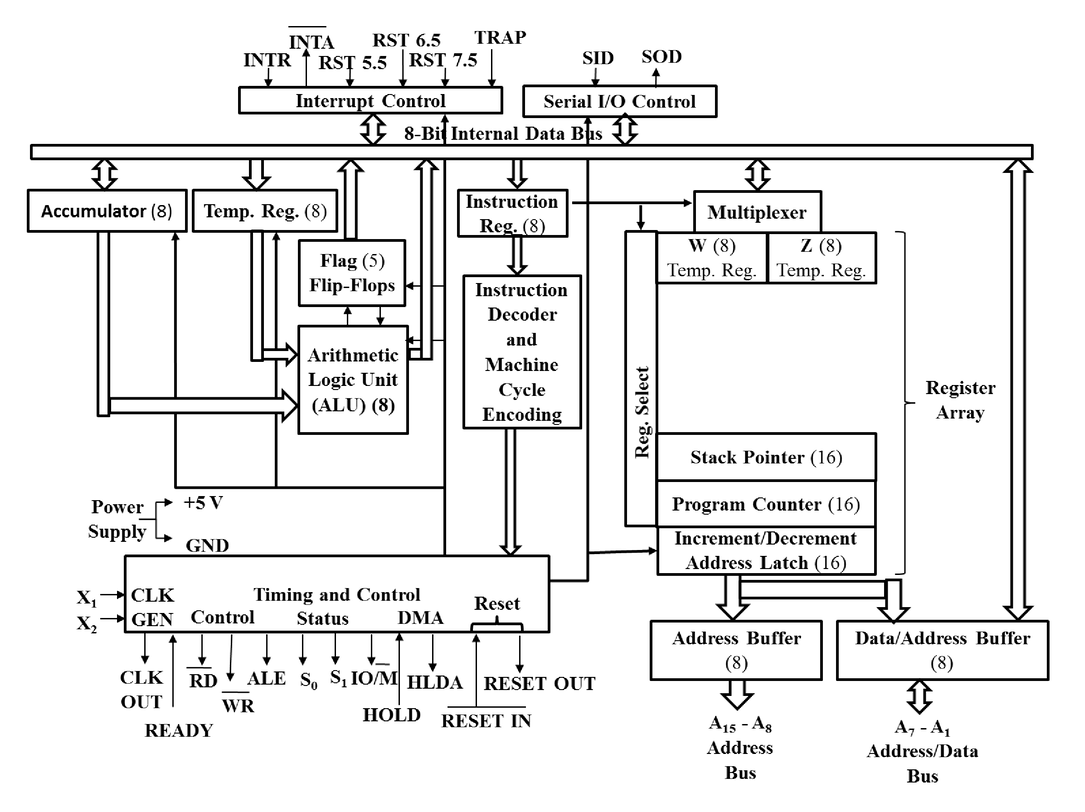
\includegraphics[width=\columnwidth]{../figs/8085architecture.png} 
\caption{Internal Architecture of 8085 MP}
\label{fig:8085}
\end{figure}


\vspace{10mm}
\section{\textbf{Code Setup}}
\begin{enumerate}
 \item Flash the following setup code through USB-UART 
 \begin{center}
\fbox{\parbox{8cm}{\url{https://github.com/KrishnaYadati/8085-programing-with-Esp32/blob/main/codes/setup/src/main.cpp}}}
\end{center}
\begin{center}
\end{center}
\begin{lstlisting}
svn co https://github.com/KrishnaYadati/8085-programing-with-Esp32/blob/main/codes/setup
cd  setup
pio run
pio run -t upload
\end{lstlisting}

after entering your wifi username and password (in quotes below)
\begin{lstlisting}
#define STASSID "..." // Add your network credentials
#define STAPSK  "..."
\end{lstlisting}
in src/main.cpp file
\item You can notice that Esp will be connnected to the network credentials provided above.Connect your laptop to the same network ,You should be able to find the ip address of your Esp on laptop using 
\begin{lstlisting}
ifconfig
nmap -sn 192.168.208.0/24
\end{lstlisting}
where your computer's ip address is the output of ifconfig and given by 192.168.208.x
\item Assuming that the username is computer and password is 123, flash the following code wirelessly
\begin{center}
\fbox{\parbox{8cm}{\url{https://github.com/KrishnaYadati/8085-programing-with-Esp32/blob/main/codes/ota/src/main.cpp}}}
\end{center}
through 
\begin{lstlisting}
pio run 
pio run -t nobuild -t upload --upload-port ip_addres_of_esp
\end{lstlisting}
where you may replace the above ip address with the ip address of your Esp.
\end{enumerate}

\end{document}